\begin{figure*}
\begin{subfigure}{0.5\textwidth}
    \centering
    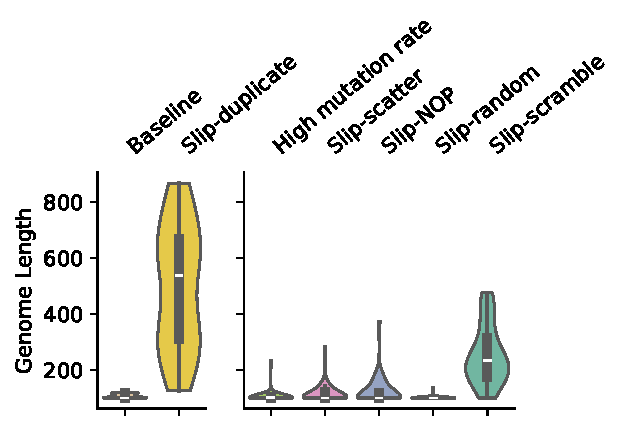
\includegraphics[width=\linewidth]{binder/binder/teeplots/col=split+env=static+hue=treatment+inner=box+kind=violin+palette=set2-r+viz=catplot+x=treatment+y=genome-length+ext=.pdf}%
    \caption{\small genome size}
    \label{fig:ablation-site-counts:genome-size}
\end{subfigure}%
\begin{subfigure}{0.5\textwidth}
    \centering
    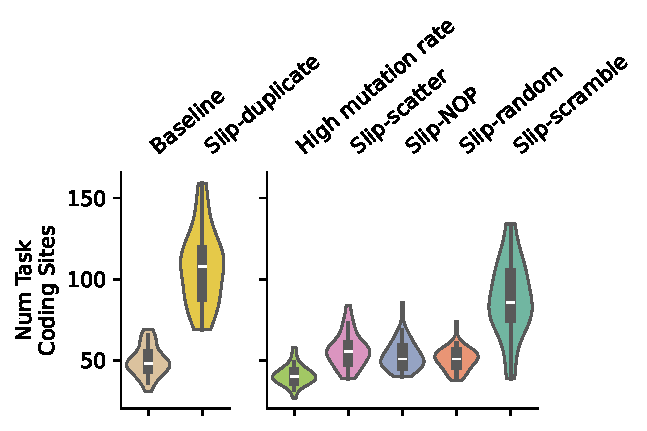
\includegraphics[width=\linewidth]{binder/binder/teeplots/col=split+env=static+hue=treatment+inner=box+kind=violin+palette=set2-r+viz=catplot+x=treatment+y=num-coding-sites+ext=.pdf}%
    \caption{\small num task coding sites}
    \label{fig:ablation-site-counts:coding-site-counts}
\end{subfigure}
\caption{
    \textbf{Genome size and task coding site count outcomes across slip-duplication ablation treatments.}
    \small Violin plots show genome size (panel \ref{fig:ablation-site-counts:coding-site-counts}) and number of task coding sites (panel \ref{fig:ablation-site-counts:coding-site-counts}) in final dominant genotypes.
    % https://github.com/chaynes2019/AvidaGeneDupe/blob/ecb7a0506d4233e57c0f7002b19ea09008dba847/binder/fig-3-static-genomelength.ipynb
    % https://github.com/chaynes2019/AvidaGeneDupe/blob/ecb7a0506d4233e57c0f7002b19ea09008dba847/binder/fig-3-static-num-coding-sites.ipynb
    Two-tailed Kruskal-Wallis tests indicate significant between-treatment variation in both genome size ($H = 130$, $p << 0.001$) and number of task coding sites ($H = 135$, $p << 0.001$).
    After applying Bonferroni correction for three comparisons, two-tailed Mann-Whitney tests confirm that genome sizes are significantly smaller under the Slip-NOP treatment compared to Slip-scramble (124 $\pm$ SD 54 vs. 252 $\pm$ SD 105 sites, $U = 814$, $p < 0.001$) and Slip-duplication treatments (124 $\pm$ SD 54 vs. 491 $\pm$ SD 223 sites, $U = 877$, $p < 0.001$); genome sizes are also significantly smaller under the Slip-scramble treatment compared to Slip-duplication ($U = 734$, $p < 0.001$).
    Similarly, the number of coding sites for metabolic tasks is significantly smaller under the Slip-NOP treatment compared to Slip-scramble (54 $\pm$ SD 10 vs. 88 $\pm$ SD 24 sites, $U = 811$, $p < 0.001$) and Slip-duplication treatments (54 $\pm$ SD 10 vs. 107 $\pm$ SD 23 sites, $U = 894$, $p < 0.001$); the number of task coding sites is also significantly smaller under the Slip-scramble treatment compared to Slip-duplication ($U = 654$, $p < 0.01$).
    }
    \label{fig:ablation-site-counts}
\end{figure*}
